% ─── Slide: How analog optical inference looks (Fig1) ────────────────────────
\begin{frame}{How analog optical inference looks}

  \vspace*{\fill}
  \begin{center}
    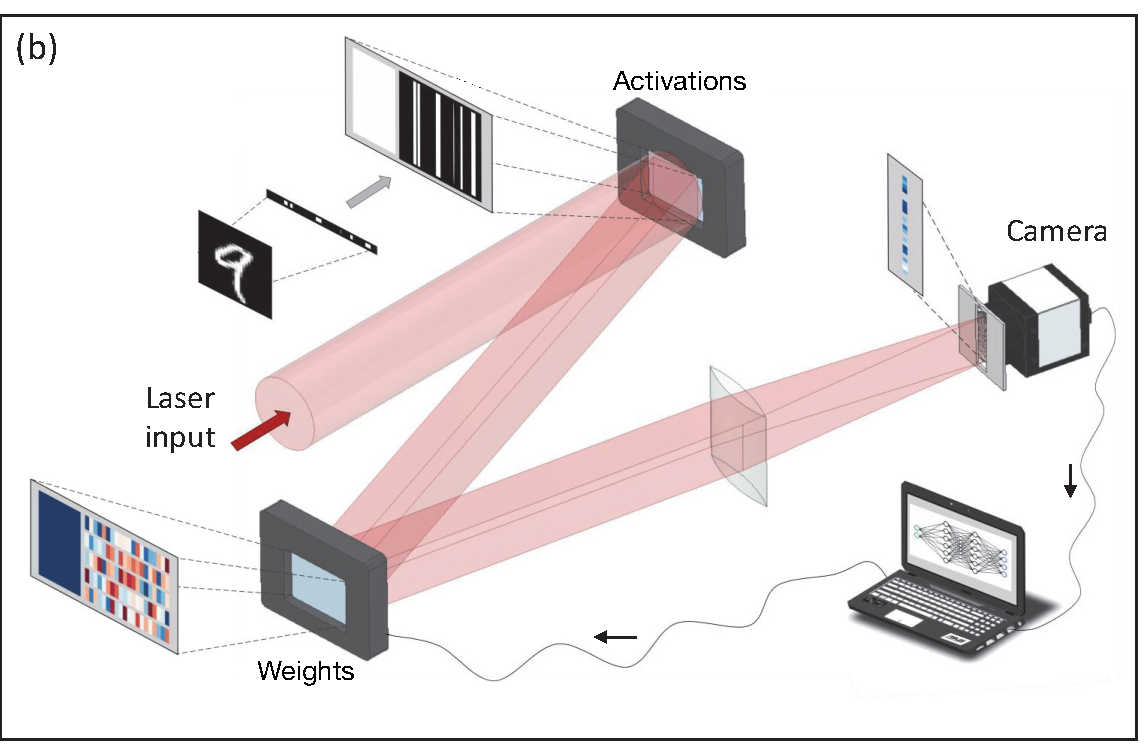
\includegraphics[height=0.78\textheight,keepaspectratio]{figs/Fig1b.pdf}
  \end{center}
  \vspace*{\fill}

  \begin{tikzpicture}[remember picture, overlay]
    \node[anchor=south west, inner sep=0pt]
      at ([xshift=0.6cm, yshift=0.35cm]current page.south west) {%
      {\tiny\color{mygray}%
        Figure adapted from \href{https://arxiv.org/abs/2203.11207}{Spall et al.,
        \textit{Hybrid training of optical neural networks},
        arXiv:2203.11207}}};
  \end{tikzpicture}

\end{frame}
